\subsubsection{Ý tưởng}
\textbf{Heap Sort} là thuật toán sắp xếp dựa trên cấu trúc dữ liệu \textbf{Binary Heap}, trong đó phần tử lớn nhất (hoặc nhỏ nhất) được đưa về gốc của \textit{heap} (\textit{max heap} hoặc \textit{min heap}). Sau đó, phần tử này được hoán đổi với phần tử cuối mảng và loại bỏ khỏi \textit{heap}. Quá trình xây dựng lại \textit{heap} và hoán đổi được lặp lại cho đến khi mảng được sắp xếp.

\subsubsection{Mã giả}
\begin{algorithm}[H]
\caption{Heap Sort}
\begin{algorithmic}[1]
\Procedure{HeapSort}{$arr, n$}
    \State \textbf{Input:} Mảng $arr$ gồm $n$ phần tử
    \State \textbf{Output:} Mảng $arr$ được sắp xếp
    
    \For {$i \gets n /2 -1 $ \textbf{downto} $0$}
        \State \Call {Heapify}{$arr, n, i$}
    \EndFor
    
    \For {$i \gets n - 1$ \textbf{downto} $0$}
        \State \textbf{swap} $arr[0]$ \textbf{and} $arr[i]$
        \State \Call {heapify}{$arr, i, 0$}
    \EndFor
\EndProcedure
\Procedure{Heapify}{$arr, n, i$}
    \State $largest \gets i$
    \State $left \gets 2\times i + 1$
    \State $right \gets 2\times i + 2$
    \If {$left < n$ \textbf{and} $arr[largest] < arr[left]$}
        \State $largest \gets left$
    \EndIf
    \If {$right < n$ \textbf{and} $arr[largest] < arr[right]$}
        \State $largest \gets right$
    \EndIf
    \If {$largest \ne i$}
        \State \textbf{swap} $arr[i]$ \textbf{and} $arr[largest]$
        \State \Call {heapify}{$arr, n, largest$}
    \EndIf
\EndProcedure
\end{algorithmic}
\end{algorithm}

\subsubsection{Ví dụ}
Dưới đây là các bước chạy tay của thuật toán \textbf{Heap Sort}:

\begin{itemize}
    \item [\textbf{--}] Đầu tiên chúng ta sẽ xây dựng \textbf{max heap}:
\end{itemize}

\begin{figure}[H]
    \centering
    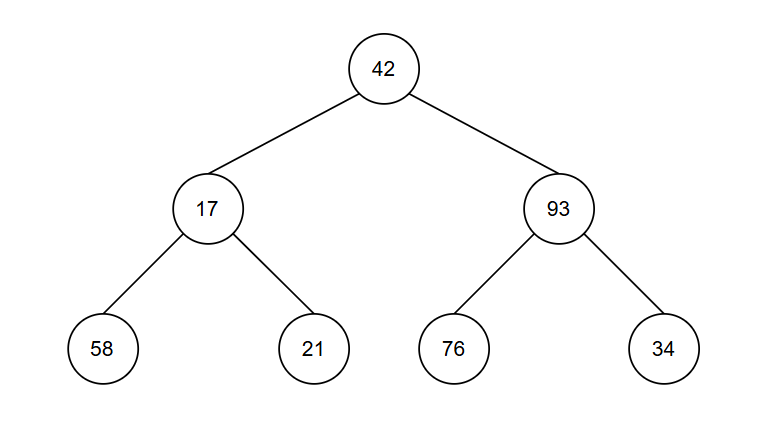
\includegraphics[width=0.5\linewidth]{img/heap_sort/1.png}
    \vspace{0.01cm}

    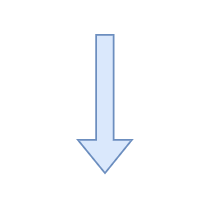
\includegraphics[width=0.1\linewidth]{img/heap_sort/arrow.png}
    \vspace{0.01cm}

    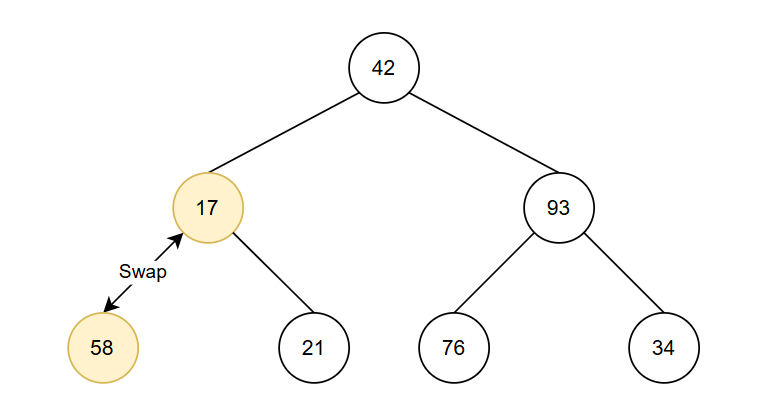
\includegraphics[width=0.5\linewidth]{img/heap_sort/2.png}
    \vspace{0.01cm}

    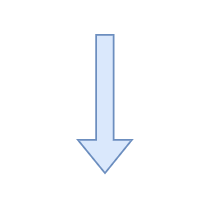
\includegraphics[width=0.1\linewidth]{img/heap_sort/arrow.png}
    \vspace{0.01cm}

    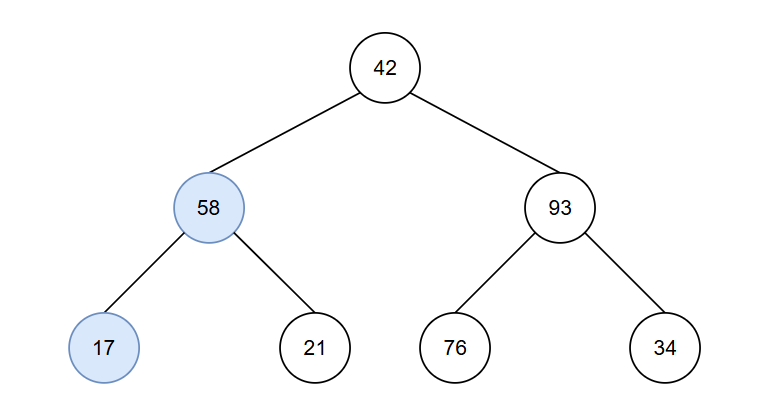
\includegraphics[width=0.5\linewidth]{img/heap_sort/3.png}

    \caption{Các bước xây dựng \textit{max heap} - 1}
\end{figure}

\begin{figure}[H]
    \centering
    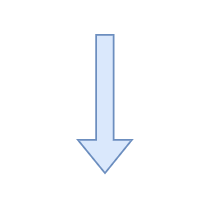
\includegraphics[width=0.1\linewidth]{img/heap_sort/arrow.png}
    \vspace{0.01cm}

    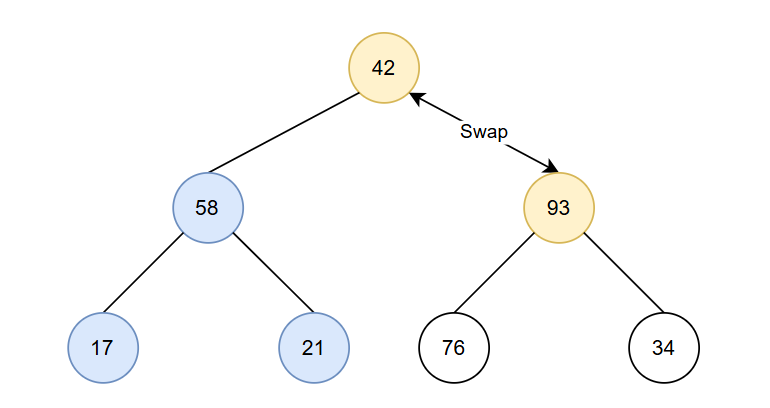
\includegraphics[width=0.5\linewidth]{img/heap_sort/4.png}
    \vspace{0.01cm}

    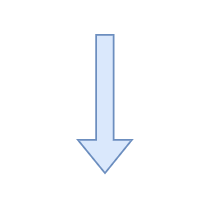
\includegraphics[width=0.1\linewidth]{img/heap_sort/arrow.png}
    \vspace{0.01cm}
    
    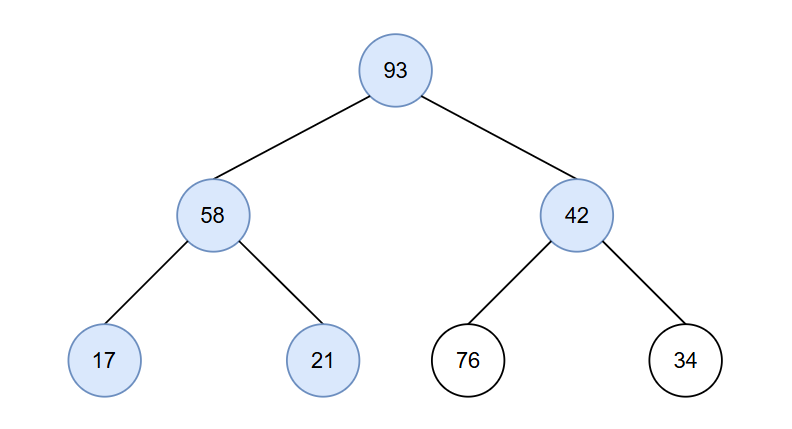
\includegraphics[width=0.5\linewidth]{img/heap_sort/5.png}
    \vspace{0.01cm}

    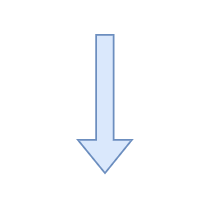
\includegraphics[width=0.1\linewidth]{img/heap_sort/arrow.png}
    \vspace{0.01cm}

    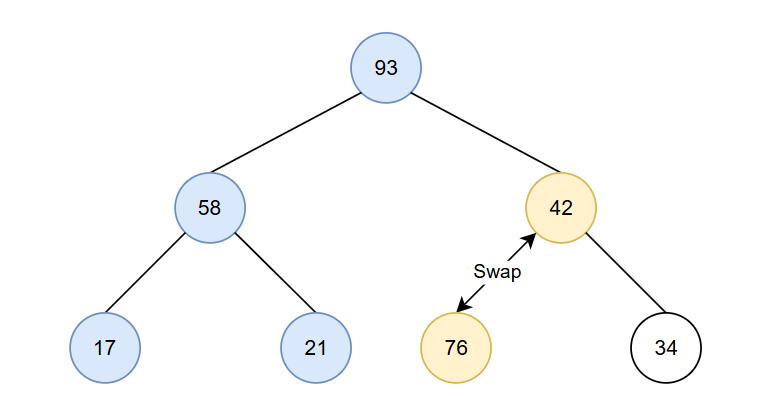
\includegraphics[width=0.5\linewidth]{img/heap_sort/6.png}

    \caption{Các bước xây dựng \textit{max heap} - 2}
\end{figure}

\begin{figure}[H]
    \centering
    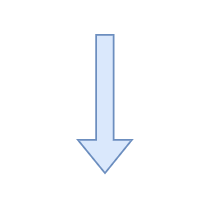
\includegraphics[width=0.1\linewidth]{img/heap_sort/arrow.png}
    \vspace{0.01cm}

    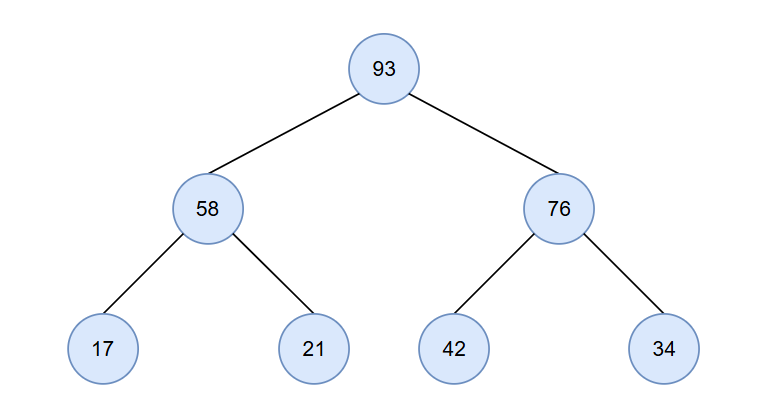
\includegraphics[width=0.5\linewidth]{img/heap_sort/7.png}

    \caption{Xây dựng thành công \textit{max heap} - 3}
\end{figure}

\begin{itemize}
    \item [\textbf{--}] Từ \textbf{max heap} vừa xây dựng ta sẽ hoán đổi phần tử ở nút gốc với phần tử cuối cùng, rồi giảm kích thước của \textbf{Heap} đi 1, sau đó thực hiện lại thao tác \textbf{Heapify} (xây dựng \textit{max heap}):
\end{itemize}

\begin{figure}[H]
    \centering
    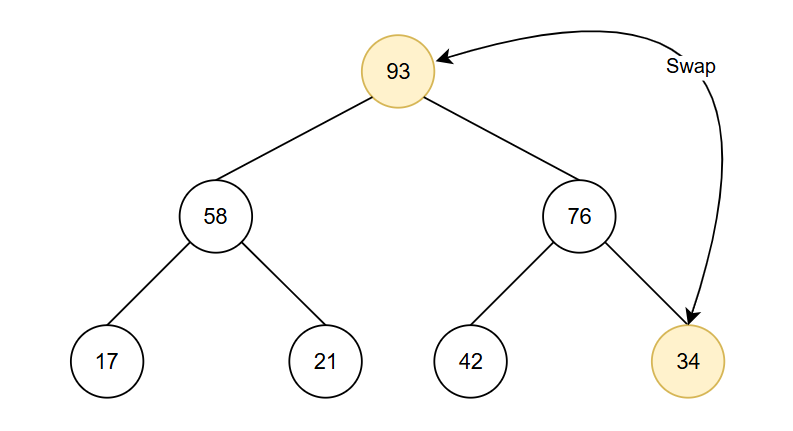
\includegraphics[width=0.5\linewidth]{img/heap_sort/8.png}
    \vspace{0.01cm}

    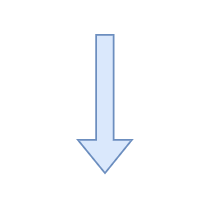
\includegraphics[width=0.1\linewidth]{img/heap_sort/arrow.png}
    \vspace{0.01cm}

    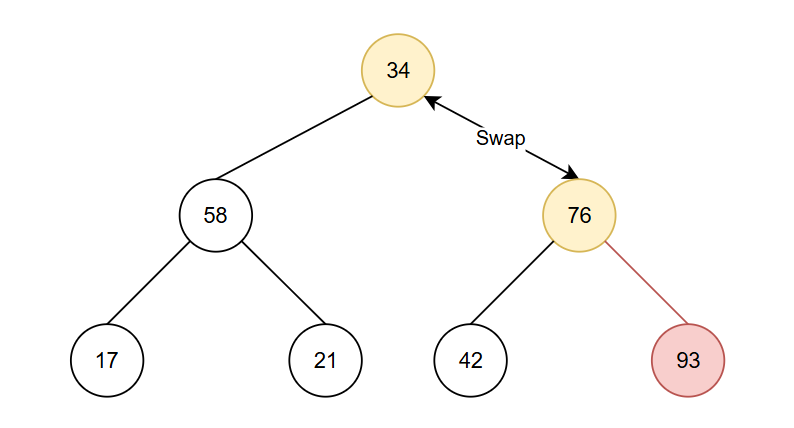
\includegraphics[width=0.5\linewidth]{img/heap_sort/9.png}

    \caption{Các bước chạy thuật toán \textbf{Heap sort} - 4}
\end{figure}

\begin{figure}[H]
    \centering
    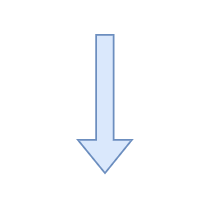
\includegraphics[width=0.1\linewidth]{img/heap_sort/arrow.png}
    \vspace{0.01cm}

    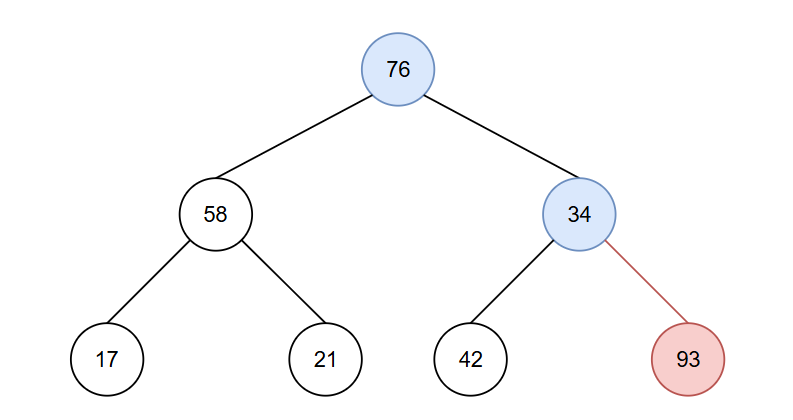
\includegraphics[width=0.5\linewidth]{img/heap_sort/10.png}
    \vspace{0.01cm}

    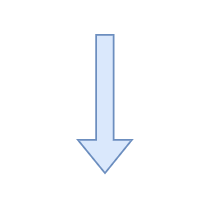
\includegraphics[width=0.1\linewidth]{img/heap_sort/arrow.png}
    \vspace{0.01cm}

    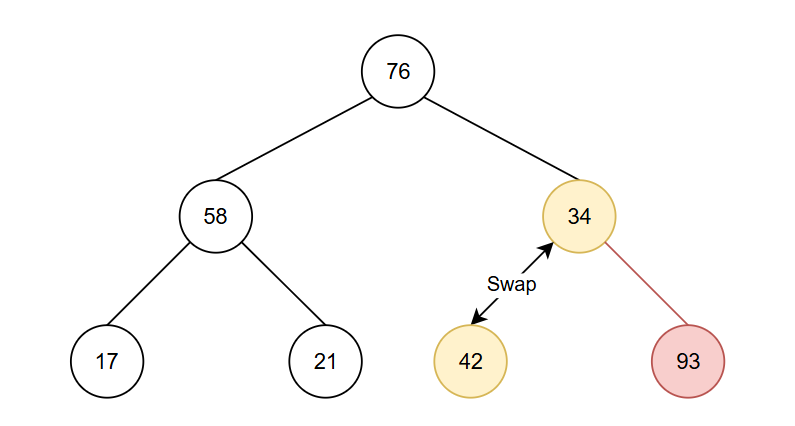
\includegraphics[width=0.5\linewidth]{img/heap_sort/11.png}
    \vspace{0.01cm}

    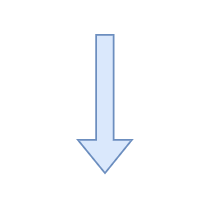
\includegraphics[width=0.1\linewidth]{img/heap_sort/arrow.png}
    \vspace{0.01cm}

    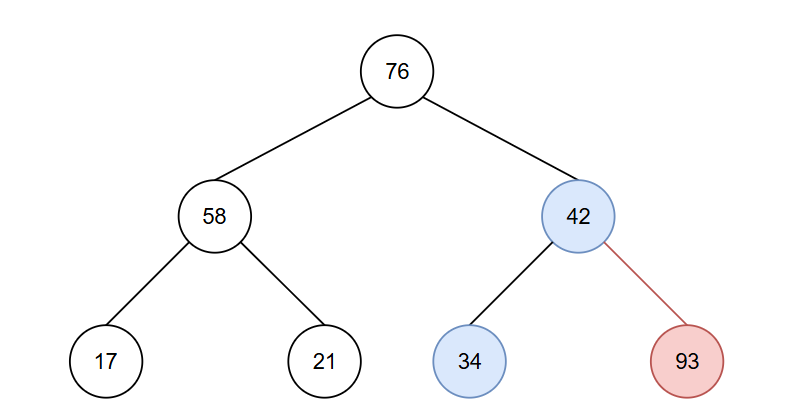
\includegraphics[width=0.5\linewidth]{img/heap_sort/12.png}

    \caption{Các bước chạy thuật toán \textbf{Heap sort} - 5}
\end{figure}

\begin{figure}[H]
    \centering
    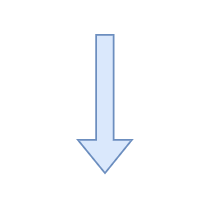
\includegraphics[width=0.1\linewidth]{img/heap_sort/arrow.png}
    \vspace{0.01cm}

    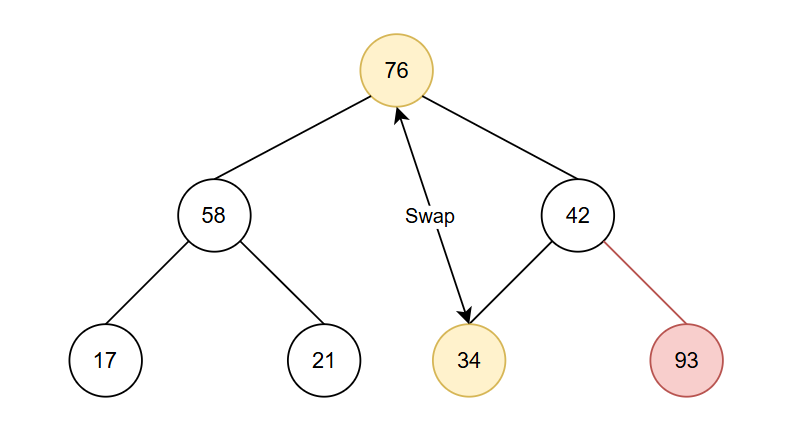
\includegraphics[width=0.5\linewidth]{img/heap_sort/13.png}
    \vspace{0.01cm}

    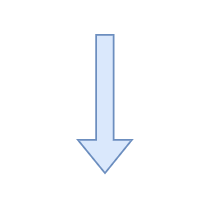
\includegraphics[width=0.1\linewidth]{img/heap_sort/arrow.png}
    \vspace{0.01cm}

    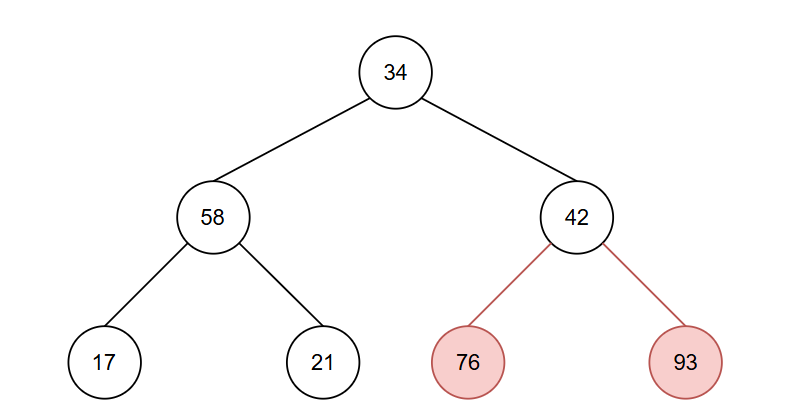
\includegraphics[width=0.5\linewidth]{img/heap_sort/14.png}
    \vspace{0.01cm}

    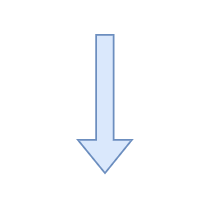
\includegraphics[width=0.1\linewidth]{img/heap_sort/arrow.png}
    \vspace{0.01cm}

    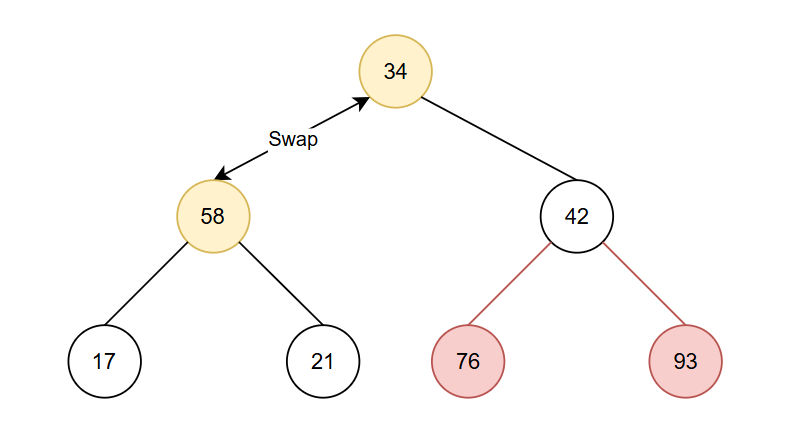
\includegraphics[width=0.5\linewidth]{img/heap_sort/15.png}

    \caption{Các bước chạy thuật toán \textbf{Heap sort} - 6}
\end{figure}

\begin{figure}[H]
    \centering
    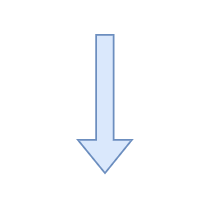
\includegraphics[width=0.1\linewidth]{img/heap_sort/arrow.png}
    \vspace{0.01cm}

    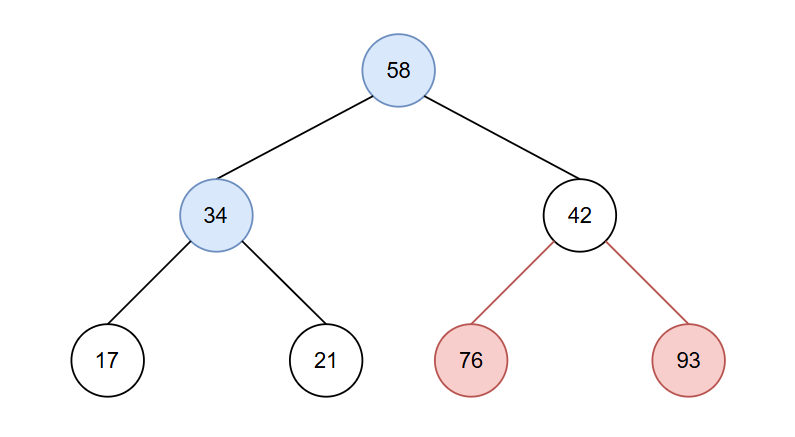
\includegraphics[width=0.5\linewidth]{img/heap_sort/16.png}
    \vspace{0.01cm}

    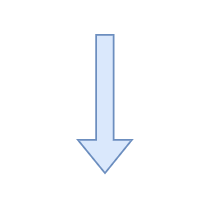
\includegraphics[width=0.1\linewidth]{img/heap_sort/arrow.png}
    \vspace{0.01cm}

    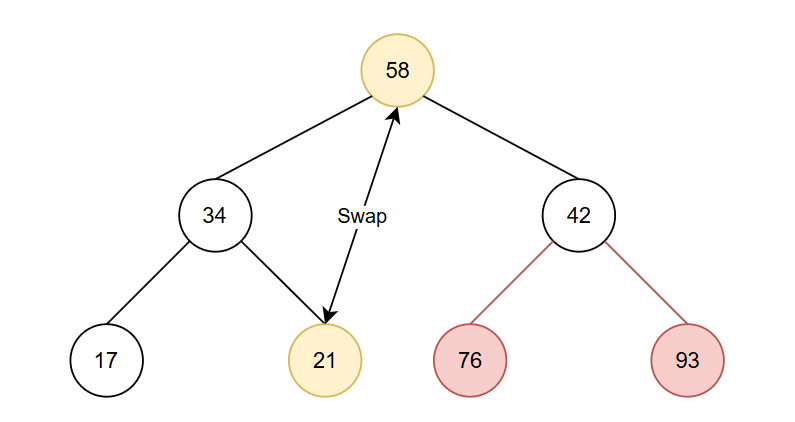
\includegraphics[width=0.5\linewidth]{img/heap_sort/17.png}
    \vspace{0.01cm}

    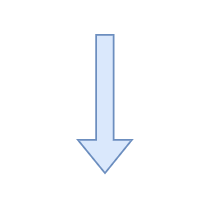
\includegraphics[width=0.1\linewidth]{img/heap_sort/arrow.png}
    \vspace{0.01cm}

    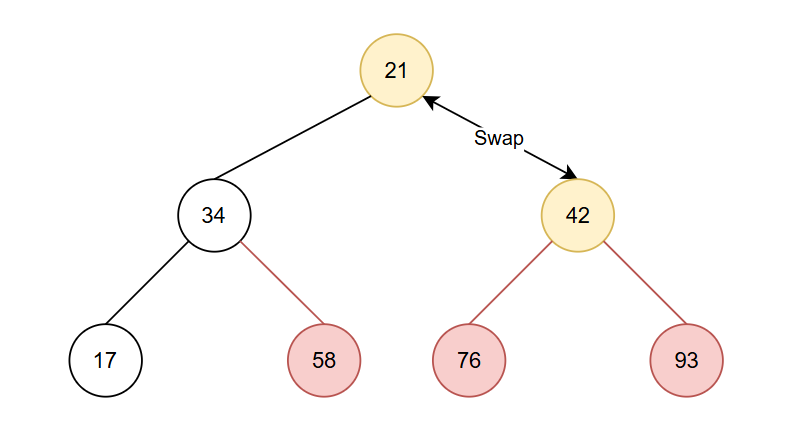
\includegraphics[width=0.5\linewidth]{img/heap_sort/18.png}

    \caption{Các bước chạy thuật toán \textbf{Heap sort} - 7}
\end{figure}

\begin{figure}[H]
    \centering
    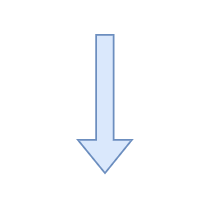
\includegraphics[width=0.1\linewidth]{img/heap_sort/arrow.png}
    \vspace{0.01cm}

    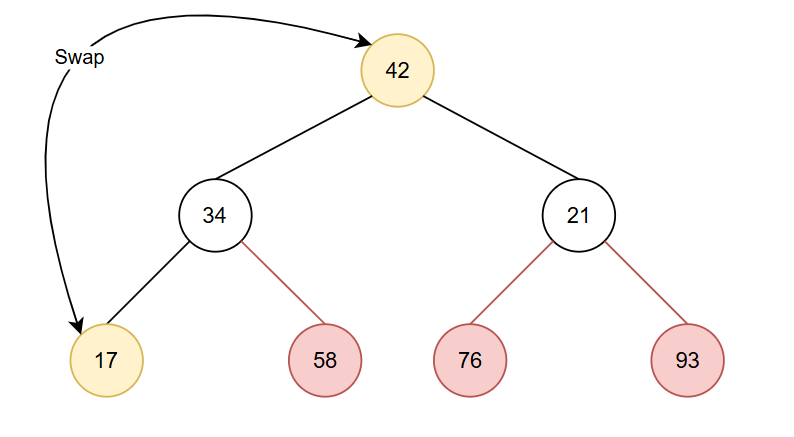
\includegraphics[width=0.5\linewidth]{img/heap_sort/19.png}
    \vspace{0.01cm}

    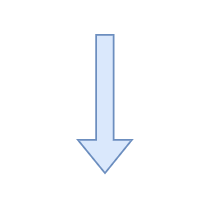
\includegraphics[width=0.1\linewidth]{img/heap_sort/arrow.png}
    \vspace{0.01cm}

    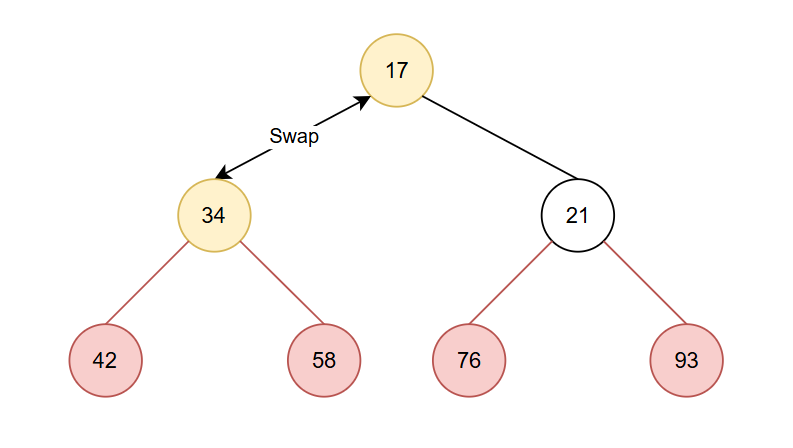
\includegraphics[width=0.5\linewidth]{img/heap_sort/20.png}
    \vspace{0.01cm}

    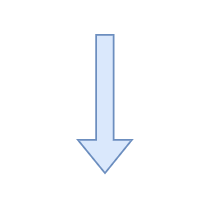
\includegraphics[width=0.1\linewidth]{img/heap_sort/arrow.png}
    \vspace{0.01cm}

    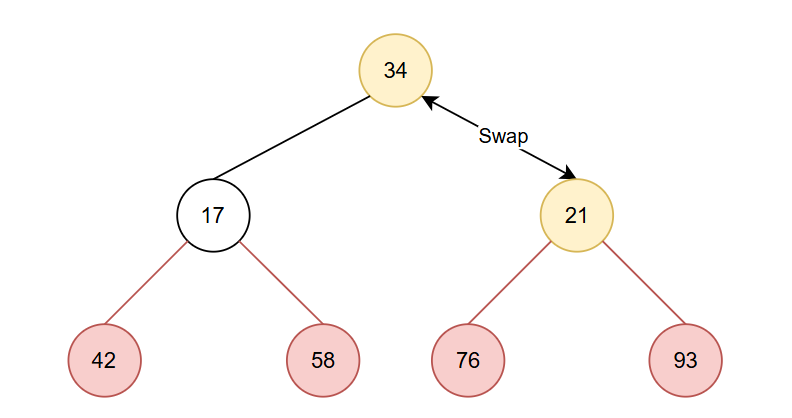
\includegraphics[width=0.5\linewidth]{img/heap_sort/21.png}

    \caption{Các bước chạy thuật toán \textbf{Heap sort} - 8}
\end{figure}

\begin{figure}[H]
    \centering
    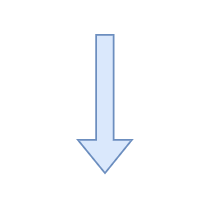
\includegraphics[width=0.1\linewidth]{img/heap_sort/arrow.png}
    \vspace{0.5cm}

    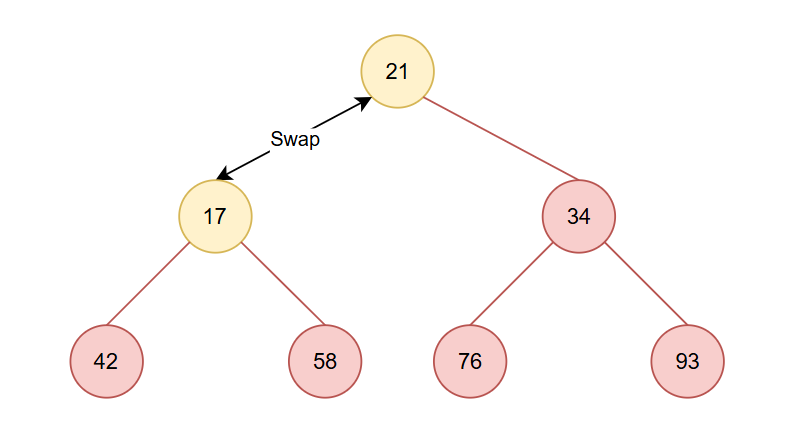
\includegraphics[width=0.5\linewidth]{img/heap_sort/22.png}
    \vspace{0.5cm}

    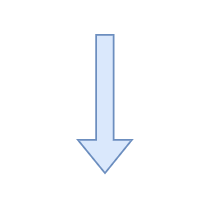
\includegraphics[width=0.1\linewidth]{img/heap_sort/arrow.png}
    \vspace{0.5cm}

    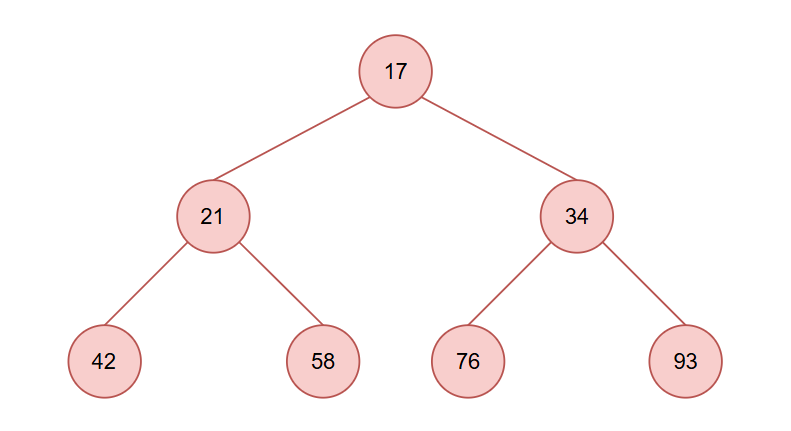
\includegraphics[width=0.5\linewidth]{img/heap_sort/23.png}

    \caption{Các bước chạy thuật toán \textbf{Heap sort} - 9}
\end{figure}
\subsubsection{Độ phức tạp}

\begin{itemize}
    \item [\textbf{--}] \textbf{Quá trình xây dựng Heap (Build Heap):}
    \begin{itemize}
        \item [$\bullet$] \textbf{Phân tích chi tiết:}
        \begin{itemize}
            \item [$\bullet$] Với mỗi nút ở cấp độ $i$, chi phí tái cấu trúc \textbf{Heap} (\textit{Heapify}) tỷ lệ với chiều cao của nút đó, $h_i$.
            \item [$\bullet$] Số lượng nút ở mỗi cấp đó $k$ của cây nhị phân là $2^k$, và chiều cao của cây là $\log n$.
            \item [$\bullet$] Tổng chi phí được tính bằng:
            \begin{center}
                $T_{\text{build}} = \sum_{k=0}^{\log n - 1} \frac{n}{2^{k+1}} \cdot k$
            \end{center}
            \item [$\bullet$] Sau khi triển khai bài toán và đơn giản hóa, ta có:
            \begin{center}
                $T_{\text{build}} = \mathcal{O}(n)$
            \end{center}
        \end{itemize}
    \end{itemize}
    \item [\textbf{--}] \textbf{Quá trình sắp xếp (Heap sort):}
    \begin{itemize}
        \item [$\bullet$] Sau khi xây dựng \textbf{Heap}, phần tử lớn nhất (gốc \textit{Heap}) được đưa về cuối mảng, và sau đó \textbf{Heapify} lại.
        \item [$\bullet$] \textbf{Chi phí tái cấu trúc Heap (\textit{Heapify}):}
        \begin{itemize}
            \item [$\bullet$] Tại mỗi bước, \textbf{Heapify} có độ phức tạp $\mathcal{O}(\log n)$.
            \item [$\bullet$] Tổng số bước là $n-1$ vì mỗi lần chỉ sắp xếp một phần tử.
            \item [$\bullet$] Tổng chi phí:
            \begin{center}
                $T_{\text{sort}} = \sum_{i=1}^{n-1} \mathcal{O}(\log i) = \mathcal{O}(n \cdot \log n)$
            \end{center}
        \end{itemize}
    \end{itemize}
    \item [\textbf{--}] \textbf{Độ phức tạp tổng quát:}
    \begin{itemize}
        \item [$\bullet$] Tổng độ phức tạp của \textbf{Heap sort} là tổng chi phí của việc xây dựng \textbf{Heap} và sắp xếp:
        \begin{center}
            $T_{\text{total}} = T_{\text{build}} + T_{\text{sort}} = \mathcal{O}(n) + \mathcal{O}(n \cdot \log n) = \mathcal{O}(n \cdot \log n)$
        \end{center}
    \end{itemize}
    \item [\textbf{--}] \textbf{Phân tích theo các trường hợp:}
    \begin{itemize}
        \item [$\bullet$] \textbf{Trường hợp tốt nhất}
        \begin{itemize}
            \item [$\bullet$] Trường hợp tốt nhất, \textbf{Heapify} vẫn phải thực hiện đầy đủ các bước, vì vậy không giảm độ phức tạp:
            \begin{center}
                $T_{\text{best}} = \mathcal{O}(n \cdot \log n)$
            \end{center}
        \end{itemize}
        \item [$\bullet$] \textbf{Trường hợp trung bình}
        \begin{itemize}
            \item [$\bullet$] Với các mảng ngẫu nhiên, sắp xếp, gần được sắp xếp, mảng giảm dần, trung bình mỗi lần \textbf{Heapify} vẫn có độ phức tạp $\mathcal{O}(\log n)$, lặp lại $n-1$ lần mà không phụ thuộc vào trạng thái ban đầu của mảng.
            \begin{center}
                $T_{\text{average}} = \mathcal{O}(n \cdot \log n)$
            \end{center}
        \end{itemize}
        \item [$\bullet$] \textbf{Trường hợp xấu nhất}
        \begin{itemize}
            \item [$\bullet$] Trường hợp xấu nhất cũng không khác biệt vì \textbf{Heapify} vẫn phải xử lý toàn bộ chiều của \textbf{Heap}.
            \begin{center}
                $T_{\text{worst}} = \mathcal{O}(n \cdot \log n)$
            \end{center}
        \end{itemize}
    \end{itemize}
    \item [\textbf{--}] \textbf{Không gian bộ nhớ:}
    \begin{itemize}
        \item [$\bullet$] \textbf{Heap sort} sử dụng \textbf{\textit{Heap in-place}} (trong cùng mảng), vì vậy độ phức tạp không gian là:
        \begin{center}
            $S = \mathcal{O}(1)$
        \end{center}
    \end{itemize}
    \item [\textbf{--}] \textbf{Độ ổn đinh:}
    \begin{itemize}
        \item [$\bullet$] \textbf{Heap sort không ổn định} vì quá trình hoán đổi giữa các phần tử có giá trị bằng nhau có thể làm thay đổi thứ tự của chúng.
    \end{itemize}
\end{itemize}
